\section{Contraction Theory}

% ════════════════════════════════════════════════════
\subsection{What is Contraction Theory?}

\begin{frame}{\insertsubsectionhead}{}

    \textbf{Contraction Theory} is a powerful tool for analyzing the stability of nonlinear systems by examining \cblue{differential dynamics}, providing insights into the behavior of \cblue{trajectories} (not points) and their convergence properties \cite{LOHMILLER:1998aa}.

    \begin{equation} \label{eq:pre:sys}
        \ddtt\mv{x}
        =
        \mv{f}(\mv{x},t)
        \quad
        \rightarrow
        \quad
        \text{diff. dyn. }
        \ddtt{\delta\mv{x}}
        =
        \pptfrac{\mv{f}}{\mv{x}} \delta\mv{x}
        .
    \end{equation}

    % \onslide<2->
    % {
    \begin{itemize}
        \item If there exists positive definite \cblue{Contraction Metric} $\mm{M}$ such that $\ddtt V\le -\alpha V$, the system is contracting.
        \item $\delta\mv{x}$ shrinks exponentially in the Riemannian space defined by $\mm{M}$ (exponential convergence of trajectories).
    \end{itemize}

    \begin{equation} 
        \text{ Lya. func. }
        V = \delta\mv{x}^\top \mv{M}(\mv{x},t) \delta\mv{x}
        ,
        \quad
        \text{cond. for contraction }
        \ddtt\mm{M} + 2\mysym\left( \mm{M}\pptfrac{\mv{f}}{\mv{x}} \right) \le -2\alpha \mm{M}
    \end{equation}
    % }

    % \onslide<3->
    % {
    \small{
        \begin{itemize}
        \item \textbf{Exponential Convergence}: Trajectories globally exponentially converge to each other regardless of initial conditions.
        \item \textbf{Control Design}: Owing to nature of differential dynamics, \cblue{LPV control design} methods can be applied.
        \end{itemize}
    }
    % }

    \begin{figure}
        \centering
        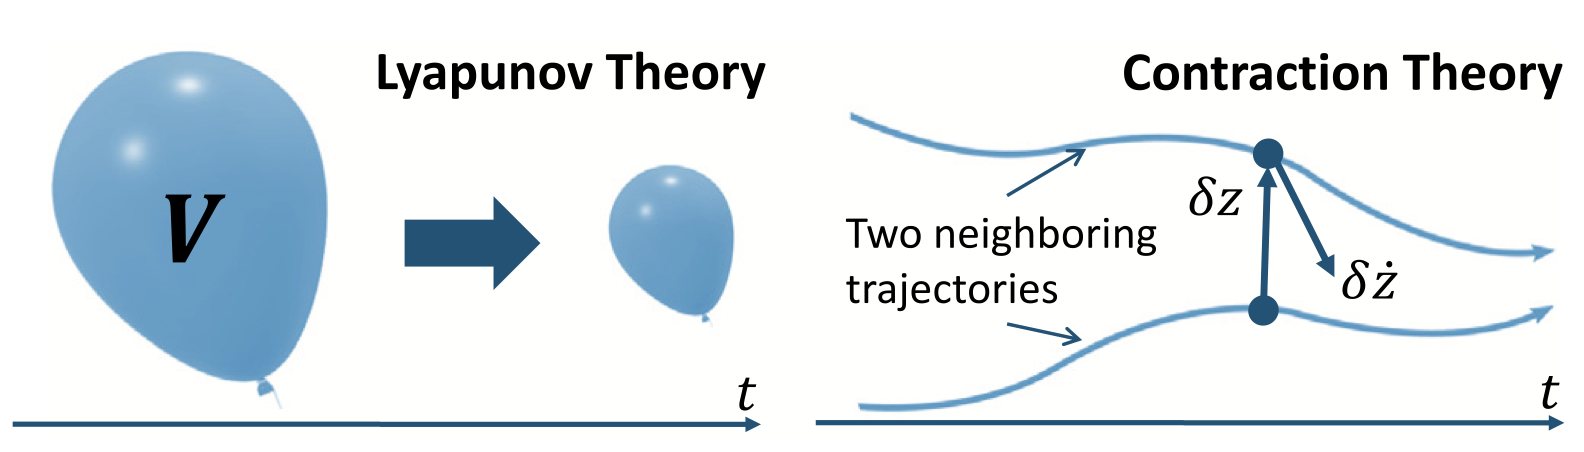
\includegraphics[width=0.45\textwidth]{figures/contraction.png}
        \caption{Lyapunov theory versus contraction theory \cite{Tsukamoto:2021aa}.}
        \label{fig:contraction:theory}
    \end{figure}

\end{frame}

\subsection{Control Contraction Metric (CCM)}

\begin{frame}{\insertsubsectionhead}{}

    \textbf{Control Contraction Metric (CCM)} is an \cblue{extension of contraction theory to control systems}, providing a framework for designing stabilizing controllers \cite{Manchester:2017aa}.

    Consider a control-affine system:
    \begin{equation}    
        \ddtt\mv{x}
        =
        \mv{f}(\mv{x},t) + \mv{B}(\mv{x},t)\mv{u}
        \quad
        \rightarrow
        \quad
        \text{diff. dyn. }
        \ddtt{\delta\mv{x}}
        =
        \pptfrac{\mv{f}}{\mv{x}} \delta\mv{x} + \pptfrac{\mv{B}}{\mv{x}} \delta\mv{x} + \mv{B}\delta\mv{u}
        .
    \end{equation}

    \begin{theorem}[Control Contraction Metric (CCM) \cite{Manchester:2017aa}]
        For a given system, if there exists a bounded metric $\mm{M}(\mv{x},t)$ such that holds 
    \begin{equation}
        \ddtt\mm{M} + 2\mysym\left( \mm{M}\pptfrac{\mv{f}}{\mv{x}} + \pptfrac{\mv{B}}{\mv{x}}\mm{M} \right) \le -2\alpha \mm{M}
        ,
    \end{equation}
    for all $\delta\mv{x}\neq 0$ such that $\delta\mv{x}^\top \mm{M}\mv{B} = 0$, then the system is \cred{universally exponentially stabilizable} via state feedback.
    \end{theorem}

    \begin{columns}
        \column{0.5\textwidth}     

    By using $\mm{M}$, a feedback controller $\mv{u}$ can be established considering the closest point on the \cblue{geodesic} between the current state and the target state in the \cred{Riemannian space} defined by $\mm{M}$, \ie $\delta\mv{u} = k(\mv{x},\delta\mv{x}, u, t)$.

        \column{0.5\textwidth}     

    \begin{figure}
        \centering
        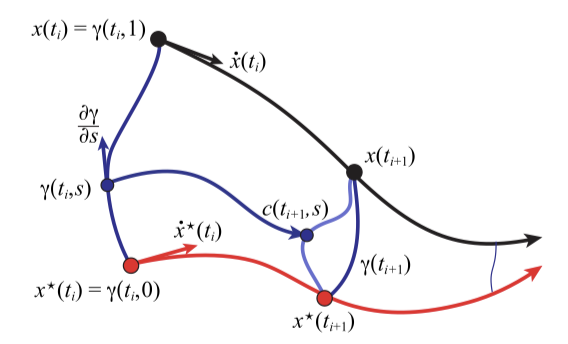
\includegraphics[width=0.45\textwidth]{figures/CCM.png}
        \caption{Control Contraction Metric (CCM) \cite{Manchester:2017aa}.}
        \label{fig:contraction:ccm}
    \end{figure}    

    \end{columns}

\end{frame}

\begin{frame}{\insertsubsectionhead}{Similiarity between CCM and CLF}

    CCM is similar to the control Lyapunov function (CLF) in that it provides a condition for the existence of a stabilizing controller.

    \begin{itemize}
        \item Both CCM and CLF provide conditions for the \cred{existence of stabilizing controllers}.
        \item CCM focuses on the contraction of trajectories in a Riemannian space defined by a metric $\mm{M}$, while CLF focuses on the decrease of a scalar function $V$ along system trajectories.
        % \item CCM can be seen as a generalization of CLF, where the contraction metric $\mm{M}$ plays a role similar to the Lyapunov function $V$ in CLF, but with a focus on the geometry of the state space rather than just scalar values.
    \end{itemize} 

    \hfill

    There are several limitations as follows:

    \begin{itemize}
        \item Finding a solution of CCM and CLF is non-convex and \cred{computationally expensive}, (should be solved iteratively and in advance).
        \item \cblue{Constraint handling} is not straightforward, and it is difficult to guarantee the satisfaction of constraints during the control design process.
        \item Since CCM and CLF are designed based on global stability properties, they may be \cred{conservative}.
    \end{itemize}

\end{frame}

\subsection{Alternative Way to Use Contraction Metric $\mm{M}$}

\begin{frame}{Alternative Way to Use Contraction Metric $\mm{M}$}

    By defining $\delta\mv{u} = k\  \rightarrow\  \mv{u} = K(\mv{x}-\mv{x}_d), \ K = \mv{Y}\mv{M}$, the contraction metric can be obtained by solving \cred{linear matrix inequalities (LMIs)} with decision variable $\mm{W}^{-1}:=\mm{M}$ \cite{Tsukamoto:2021ac}.

    According to Theorem 2.4 in \cite{Tsukamoto:2021aa}, by \cred{minimizing the condition number} $\chi$ of $\mm{M}$, the steady state error can be reduced.
    The LMI problem can be formulated as follows:
\begin{equation} \label{eq:opt:conv:lmi}
   \begin{matrix}
      \min_{
         \overline{\mm{W}},\chi,\nu
         } 
      \chi + \lambda \nu
      \\ 
      \vspace{-.2cm}
      \\
      \text{s.t. }
      \begin{cases}
         -
         \ddtt\overline{\mm{W}}
         +
         2\mysym(
            \mathbb{A}\overline{\mm{W}}
         )
         -
         2\nu\mm{B}\mm{R}^{-1} \mm{B}^\top 
         \preceq
         -2\alpha\overline{\mm{W}}
         ,
         \\
         \mm{I}_n
         \preceq
         \overline{\mm{W}}
         \preceq
         \chi \mm{I}_n
         ,
      \end{cases}
   \end{matrix}
\end{equation} 
    where $\mathbb{A}$ is state-dependent matrix which is employed to transform the system to LPV system, and $\overline{\mv{W}} = \nu \mv{W}$ is normalized $\mv{W}$, and $\nu$ is decision variable for magnitude of the contraction metric, and $\lambda$ is penalty parameter for $\nu$.
    
    \hfill

    The control input can be simply obtained by
    \begin{equation}
        \mv{u} = \mv{u}_d - \mv{R}^{-1}\mv{B}^\top \mm{M}(\mv{x}-\mv{x}_d)
         ,\quad
         \text{where } \mv{M} = \overline{\mm{W}}^{-1} \cdot \nu
    \end{equation}

    \hfill

    \begin{itemize}
        \item Easy to implement (point-wise convex condition).
        \item Due to the use of LMIs, it still should be solved in advance.
        \item According to the objective function, typically, $\mv{M}$ is designed to be identity matrix and $\nu$ is maximized, which results in \cred{a simple state feedback controller with a large proportional gain}.
    \end{itemize}

\end{frame}

\subsection{Summary}

\begin{frame}{\insertsubsectionhead}{Summary}

    Summary of the discussion on CCM and alternative way to use contraction metric $\mm{M}$:

    \begin{itemize}
        \item CCM is a powerful tool providing the existence of stabilizing controllers.
        \item CCM has similar problems to CLF, such as non-convexity, computational expense, and difficulty in handling constraints.
        \item An alternative way to use contraction metric $\mm{M}$ is to solve LMIs, which is easier to implement but still requires solving in advance and may lead to conservative controllers.
    \end{itemize}

    \hfill

    Our approach is \dots

    \begin{itemize}
        \item Solve the contraction problem in an online manner by transforming the contraction condition into \cred{a point-wise convex condition in vector space}.
        \item Extend the method to \cred{constrained systems}, such as input constraints and CBF-motivated constraints.
    \end{itemize}
    
\end{frame}